% Figure 1: CASF-2016 screening power
\begin{figure}[htbp]
\centering
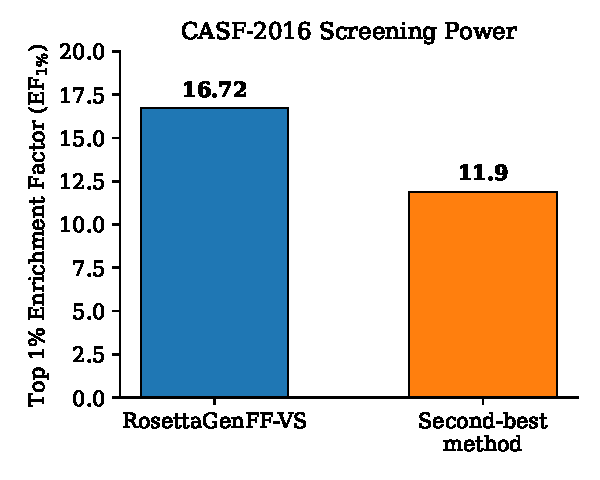
\includegraphics[width=0.55\textwidth]{figures/fig_casf_ef1.pdf}
\caption{CASF-2016 screening power comparison. Top 1\% enrichment factor
(EF$_{1\%}$) for RosettaGenFF-VS (16.72) versus the second-best method (11.9),
demonstrating a substantial margin in early-enrichment performance on the
285-complex benchmark.}
\label{fig:casf_ef1}
\end{figure}

% Figure 2: Active-learning binding affinity convergence
\begin{figure}[htbp]
\centering
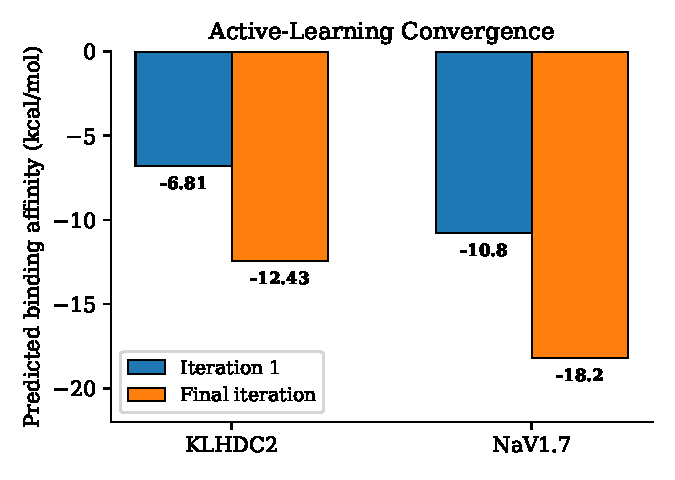
\includegraphics[width=0.6\textwidth]{figures/fig_active_learning.pdf}
\caption{Predicted binding affinity of the top 0.1 percentile compounds
across active-learning iterations for the KLHDC2 and NaV1.7 VSD4 campaigns.
KLHDC2: $-6.81$ kcal/mol (iteration~1) to $-12.43$ kcal/mol (iteration~10).
NaV1.7: $-10.8$ kcal/mol (iteration~1) to $-18.2$ kcal/mol (final iteration).}
\label{fig:active_learning}
\end{figure}

% Figure 3: Hit rates across campaigns
\begin{figure}[htbp]
\centering
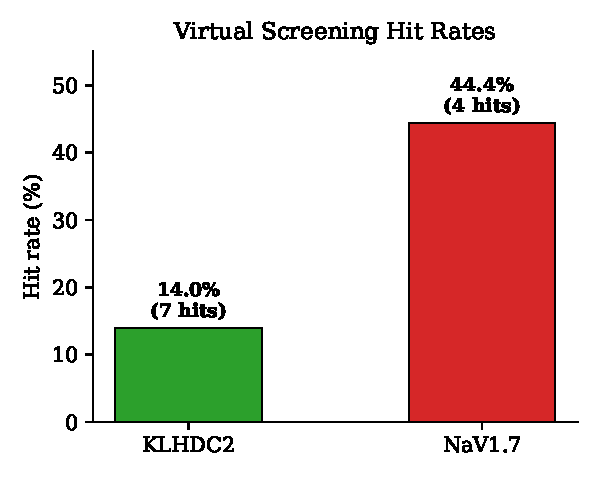
\includegraphics[width=0.55\textwidth]{figures/fig_hit_rates.pdf}
\caption{Experimental hit rates for the KLHDC2 and NaV1.7 VSD4 virtual
screening campaigns. KLHDC2: 7 hits (14\% hit rate); NaV1.7: 4 hits with
IC$_{50} < 10$~\textmu M (44.4\% hit rate).}
\label{fig:hit_rates}
\end{figure}

% Figure 4: NaV1.7 lead compound IC50 values with 95% CIs
\begin{figure}[htbp]
\centering
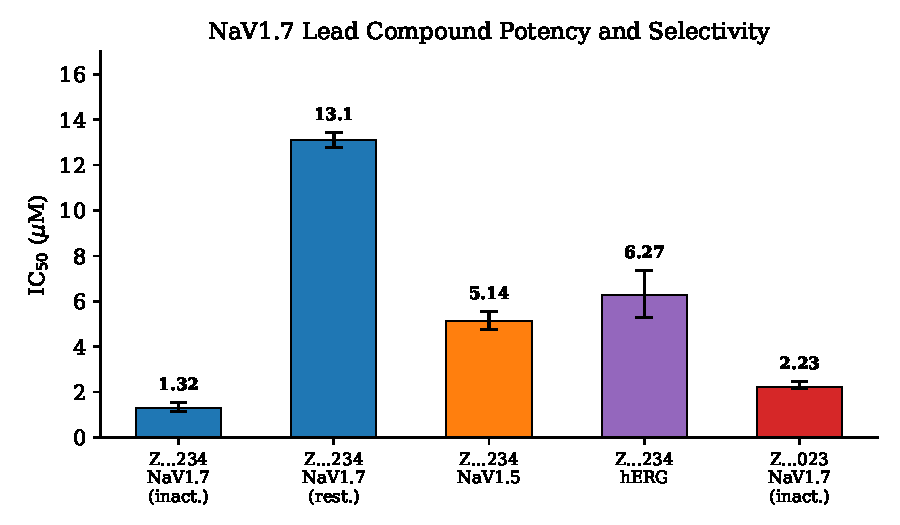
\includegraphics[width=0.7\textwidth]{figures/fig_nav17_ic50.pdf}
\caption{IC$_{50}$ values (mean, 95\% CI) for the two best NaV1.7 VSD4 lead
compounds. Z8739902234: inactivated-state IC$_{50}$ = 1.32~\textmu M
(1.14--1.55), resting-state IC$_{50}$ = 13.1~\textmu M (12.78--13.45);
selectivity against NaV1.5 (5.14~\textmu M, 4.74--5.55) and hERG
(6.27~\textmu M, 5.27--7.37). Z8739905023: inactivated-state IC$_{50}$ =
2.23~\textmu M (2.14--2.46).}
\label{fig:nav17_ic50}
\end{figure}

% Figure 5: OpenVS pipeline schematic
\begin{figure}[htbp]
\centering

\includegraphics[width=0.85\textwidth]{figures/fig_pipeline.pdf}
\caption{Schematic overview of the OpenVS platform pipeline. An ultra-large
compound library (billions of molecules) is triaged by an active-learning
neural-network surrogate, docked with VSX (fast mode), re-ranked with VSH
(flexible-receptor mode), filtered and clustered, then advanced to synthesis
and experimental assay.}
\label{fig:pipeline}
\end{figure}
